\documentclass{beamer}
\usepackage{hyperref, mathrsfs, picture, tabto, tikz, ulem}
\usecolortheme[RGB={34, 139, 34}]{structure}
\usetheme{Singapore}
\setbeamertemplate{navigation symbols}{\insertframenumber}
\definecolor{dodgerblue}{rgb}{0.12, 0.56, 1.0}
\definecolor{darkorange}{rgb}{1.0, 0.55, 0.0}
\definecolor{forestgreen}{rgb}{0.13, 0.55, 0.13}

\def\A{\mathcal A}\def\B{\mathcal B}\def\C{\mathcal C}\def\D{\mathcal D}
\def\E{\mathcal E}\def\F{\mathcal F}\def\G{\mathcal G}\def\J{\mathcal J}
\def\L{\mathcal L}\def\M{\mathcal M}\def\N{\mathcal N}\def\O{\mathcal O}
\def\P{\mathcal P}\def\Q{\mathcal Q}\def\R{\mathcal R}\def\S{\mathcal S}
\def\T{\mathcal T}\def\W{\mathcal W}\def\V{\mathcal V}\def\X{\mathcal X}
\def\Y{\mathcal Y}\def\Z{\mathcal Z}
\def\mE{\mathbb E}\def\mN{\mathbb N}\def\mP{\mathbb P}\def\mR{\mathbb R}
\def\mS{\mathbb S}
\def\bE{{\bf E}}
\def\bx{{\bf x}}
\def\prob{\mbox{\bf prob}}\def\tr{\mbox{\bf tr}}
\def\l{\left}\def\r{\right}\def\lf{\lfloor}\def\rf{\rfloor}
\def\un{\underline}
\def\theat{\theta}\def\lambad{\lambda}\def\lamda{\lambda}
\def\iid{\stackrel{\mbox{\scriptsize i.i.d.}}{\sim}}
\def\ind{\stackrel{\mbox{\scriptsize ind.}}{\sim}}
\def\minimize{\mbox{minimize}\hspace{4mm}}
\def\maximize{\mbox{maximize}\hspace{4mm}}
\def\subjectto{\mbox{subject to}\hspace{4mm}}

\title{True wOBA:\\
    \small Estimation of true talent level for batters}
\author{Scott Powers and Eli Shayer}
\institute{Stanford University}
\date{2016 SABR Analytics Conference}
\begin{document}

\begin{frame}
\titlepage
\hfill
\includegraphics[width = 1in]{../figs/ssac.png}
\end{frame}

\begin{frame}{Which statistic is more volatile?}
\begin{columns}
\begin{column}{0.5\textwidth}
\centering
{\Huge\tt BABIP}\\
$$\frac{\mbox{\tt H - HR}}{\mbox{\tt AB - K - HR + SF}}$$
~\\
\vspace{4mm}
``Stabilizes'' after 820 BIP\\
~\\
League average: .299
\end{column}
\begin{column}{0.5\textwidth}
\centering
{\Huge\tt OBP}\\
$$\frac{\mbox{\tt H + BB + HBP}}{\mbox{\tt AB + BB + HBP + SF}}$$
~\\
\vspace{4mm}
``Stabilizes'' after 460 PA\\
~\\
League average: .317
\end{column}
\end{columns}
\vspace{6.5mm}
~\\
\end{frame}

\begin{frame}{Which statistic is more volatile?}
\begin{columns}
\begin{column}{0.5\textwidth}
\centering
{\Huge\tt BABIP}\\
$$X_1 = \mbox{BABIP on $1^{st}$ 150 BIP}$$
$$X_2 = \mbox{BABIP on $2^{nd}$ 150 BIP}$$
\end{column}
\begin{column}{0.5\textwidth}
\centering
{\Huge\tt OBP}\\
$$Y_1 = \mbox{OBP on $1^{st}$ 150 PA}$$
$$Y_2 = \mbox{OBP on $2^{nd}$ 150 PA}$$
\end{column}
\end{columns}
\centering
\vspace{1cm}
Which is greater: $\mE(X_1 - X_2)^2$ or $\mE(Y_1 - Y_2)^2$?\\
~\\
\begin{columns}
\begin{column}{0.5\textwidth}
\pause
$$\sqrt{\mE(X_1 - X_2)^2} = 0.058$$
\end{column}
\begin{column}{0.5\textwidth}
\pause
$$\sqrt{\mE(Y_1 - Y_2)^2} = 0.062$$
\end{column}
\end{columns}
\end{frame}

\begin{frame}{What is going on?}
Suppose a statistic $Z$ can be split into talent $T$ and luck $L$:
$$Z_1 = T + L_1 \hspace{1cm} Z_2 = T + L_2,$$
with
$$\sigma^2_T = \mbox{Var}(T) \hspace{1cm}\mbox{and}\hspace{1cm}
    \sigma^2_L = \mbox{Var}(L_1) = \mbox{Var}(L_2)$$
\vspace{4mm}
~\\
Assuming $T$, $L_1$ and $L_2$ are independent,
$$\mbox{Corr}(Z_1, Z_2) = \frac{\sigma^2_T}{\sigma^2_T + \sigma^2_L}$$
\end{frame}

\begin{frame}{Outline}
\begin{itemize}
\item Introduction
\tabto*{8cm}\makebox(0,0){\put(0, -2\normalbaselineskip){$\left.
    \rule{0pt}{1\normalbaselineskip}\right\}$ Eli}}
\begin{itemize}
    \item Regression to the mean
\end{itemize}
\item Methods
\tabto*{8cm}\makebox(0,0){\put(0, -4.6\normalbaselineskip){$\left.
    \rule{0pt}{2\normalbaselineskip}\right\}$ Scott}}
\begin{itemize}
    \item Regularization as regression to the mean
    \item True wOBA
    \item Regularization vs. random effect models
\end{itemize}
\item Results
\tabto*{8cm}\makebox(0,0){\put(0, -4.8\normalbaselineskip){$\left.
    \rule{0pt}{2\normalbaselineskip}\right\}$ Eli}}
\begin{itemize}
    \item Validation
    \item Results on 2015 MLB regular season
\end{itemize}
\item Discussion
\end{itemize}
\end{frame}

\begin{frame}{Regression to the mean}
$$T \sim \N(\mu_T, \sigma^2_T) \hspace{1cm}
Z|T \sim \N(T, \sigma^2_L)$$
\begin{center}
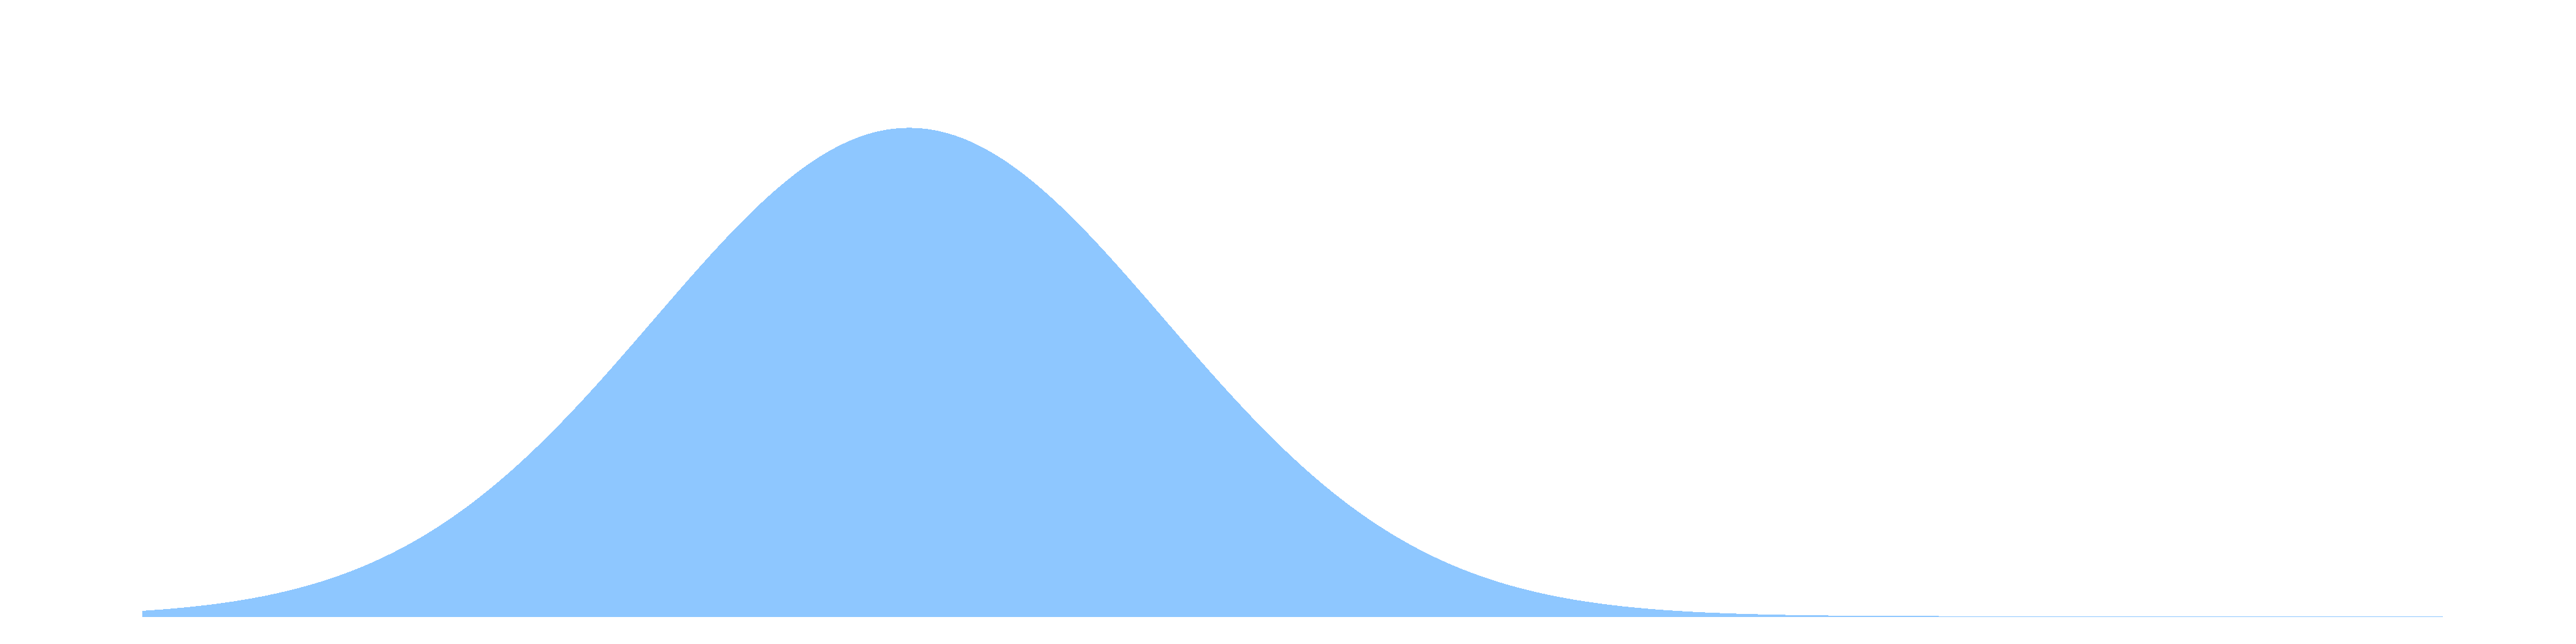
\includegraphics[width = \textwidth]{../figs/talent.pdf}\\
\end{center}
\vspace{-6mm}\tabto*{37mm}$\uparrow$\\
\tabto*{36mm}$\mu_T$
\pause
\vspace{-5mm}\tabto*{58mm}$\uparrow$\\
\tabto*{57.5mm}$Z$
{\color{white}
\vspace{-4.5mm}\tabto*{44mm}$\uparrow$\\
\tabto*{43mm}$Z^*$\\}
$${\color{white} Z^* = E[T|Z] = \frac{\sigma_T^{-2}\mu_T + \sigma_L^{-2}Z}
    {\sigma_T^{-2} + \sigma_L^{-2}} }$$
\end{frame}

\begin{frame}{Regression to the mean}
$$T \sim \N(\mu_T, \sigma^2_T) \hspace{1cm}
Z|T \sim \N(T, \sigma^2_L)$$
\begin{center}
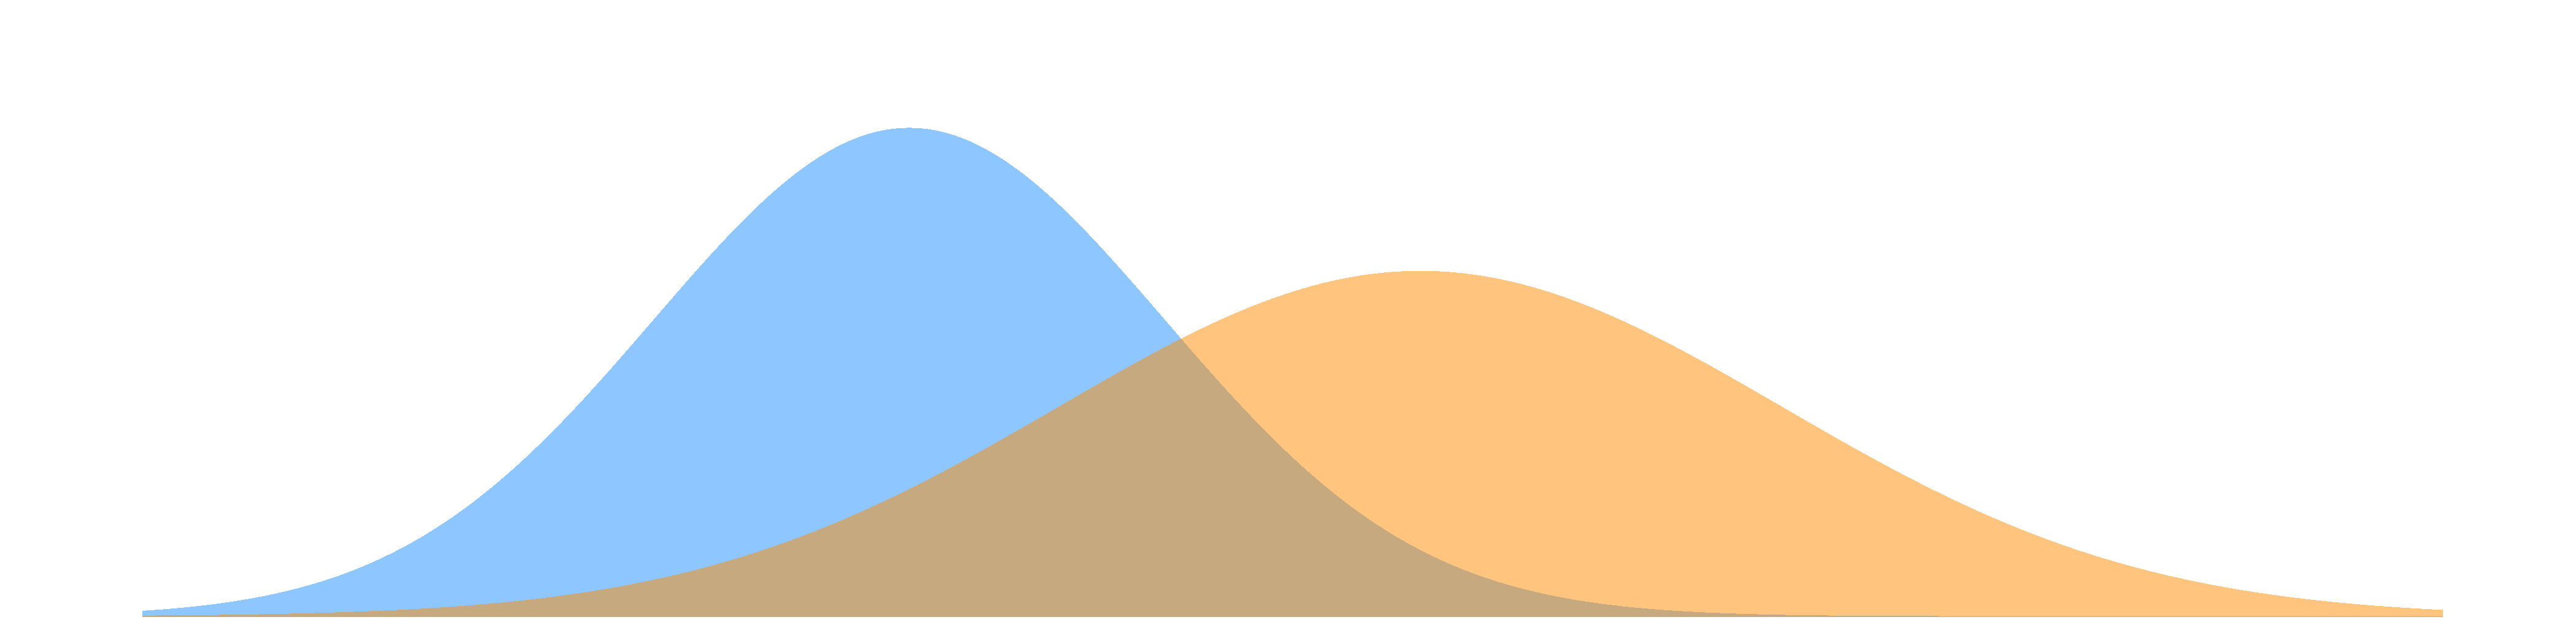
\includegraphics[width = \textwidth]{../figs/talent-skill.pdf}
\end{center}
\vspace{-6mm}\tabto*{37mm}$\uparrow$\\
\tabto*{36mm}$\mu_T$
\vspace{-5mm}\tabto*{58mm}$\uparrow$\\
\tabto*{57.5mm}$Z$
{\color{white}
\vspace{-4.5mm}\tabto*{44mm}$\uparrow$\\
\tabto*{43mm}$Z^*$\\}
$${\color{white} Z^* = E[T|Z] = \frac{\sigma_T^{-2}\mu_T + \sigma_L^{-2}Z}
    {\sigma_T^{-2} + \sigma_L^{-2}} }$$
\end{frame}

\begin{frame}{Regression to the mean}
$$T \sim \N(\mu_T, \sigma^2_T) \hspace{1cm}
Z|T \sim \N(T, \sigma^2_L)$$
\begin{center}
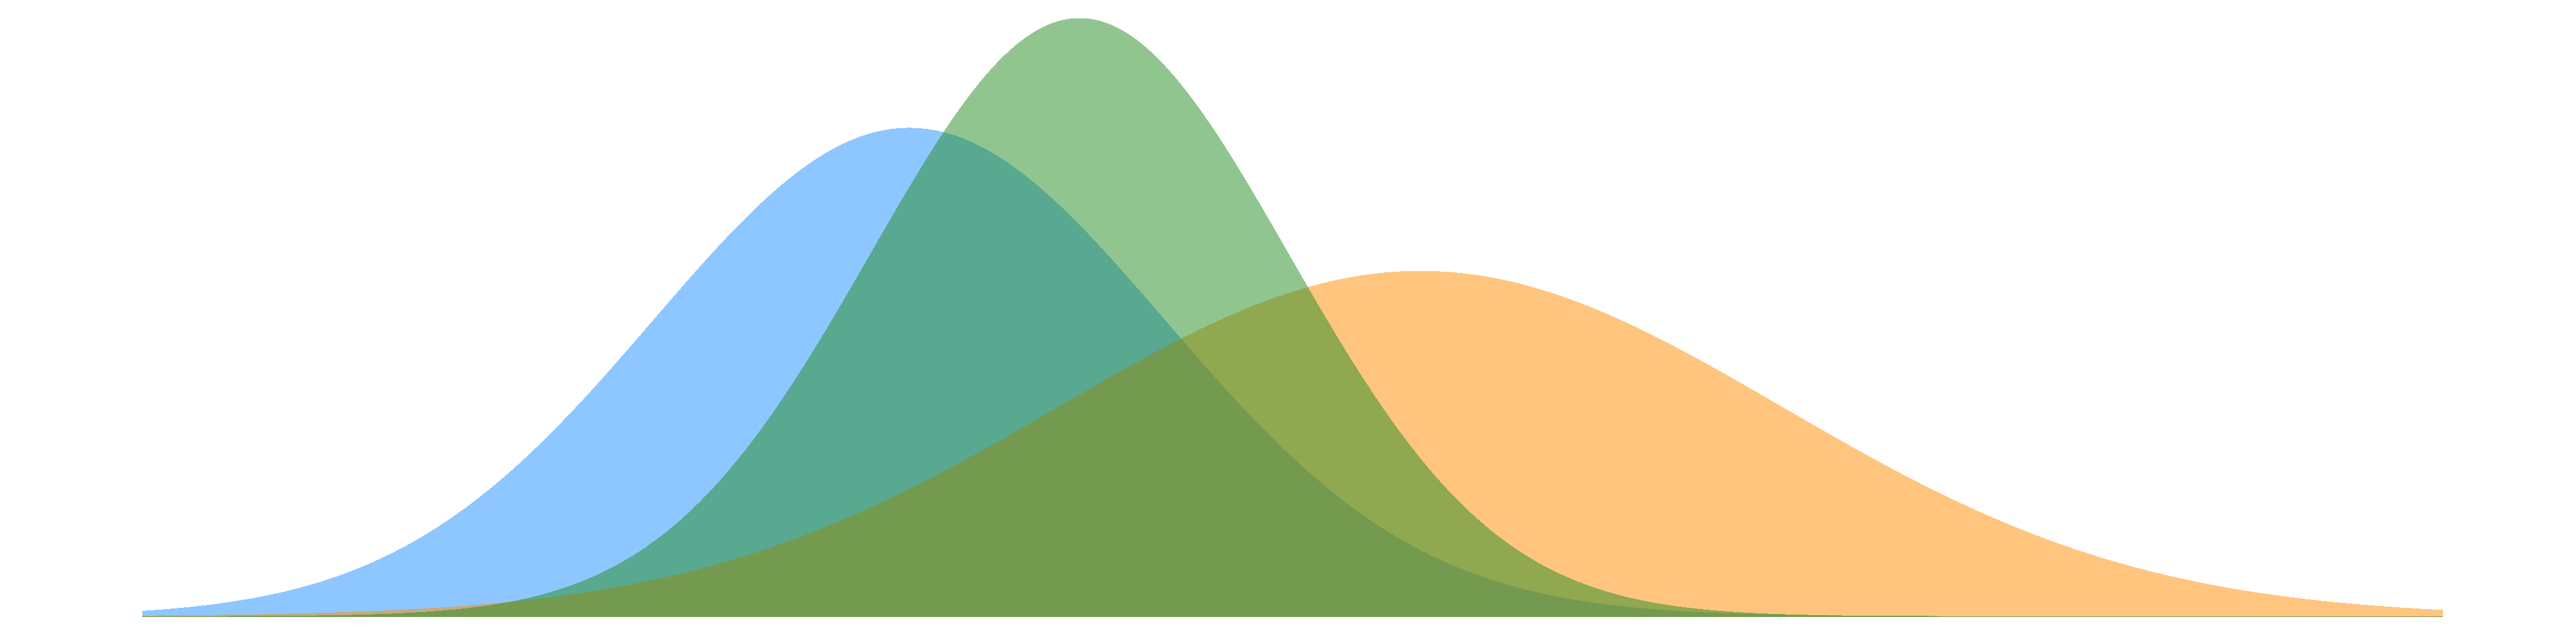
\includegraphics[width = \textwidth]{../figs/talent-skill-post.pdf}
\end{center}
\vspace{-6mm}\tabto*{37mm}$\uparrow$\\
\tabto*{36mm}$\mu_T$
\vspace{-5mm}\tabto*{58mm}$\uparrow$\\
\tabto*{57.5mm}$Z$
\vspace{-4.5mm}\tabto*{44mm}$\uparrow$\\
\tabto*{43mm}$Z^*$\\
$$Z^* = \mE[T|Z] = \frac{\sigma_T^{-2}\mu_T + \sigma_L^{-2}Z}
    {\sigma_T^{-2} + \sigma_L^{-2}}$$
\end{frame}

\begin{frame}{Regression to the mean for each outcome probability}
\centering
\begin{tabular}{c|r|cc}
\multicolumn{2}{c}{}    & (Naive)   & (Regressed)\\
    & $\hat\sigma^2_T$  & RMSE($Z$) & RMSE($Z^*$)\\
    \hline
G   & 15.85             & 4.80      & 4.42\\
F   & 20.13             & 4.45      & 4.22\\
K   & 29.10             & 4.19      & 3.89\\
BB  &  6.26             & 3.33      & 3.04\\
HBP &  0.24             & 0.94      & 0.80\\
1B  &  7.02             & 3.81      & 3.17\\
2B  &  0.45             & 2.01      & 1.62\\
3B  &  0.13             & 0.74      & 0.67\\
HR  &  1.88             & 1.79      & 1.61
\end{tabular}\\
\vspace{1cm}
{\bf Upshot}: Different population variances for different outcomes,\\
but regression to the mean improves RMSE for all of them!
\end{frame}

\begin{frame}{Regressed wOBA vs. naive wOBA}
\centering
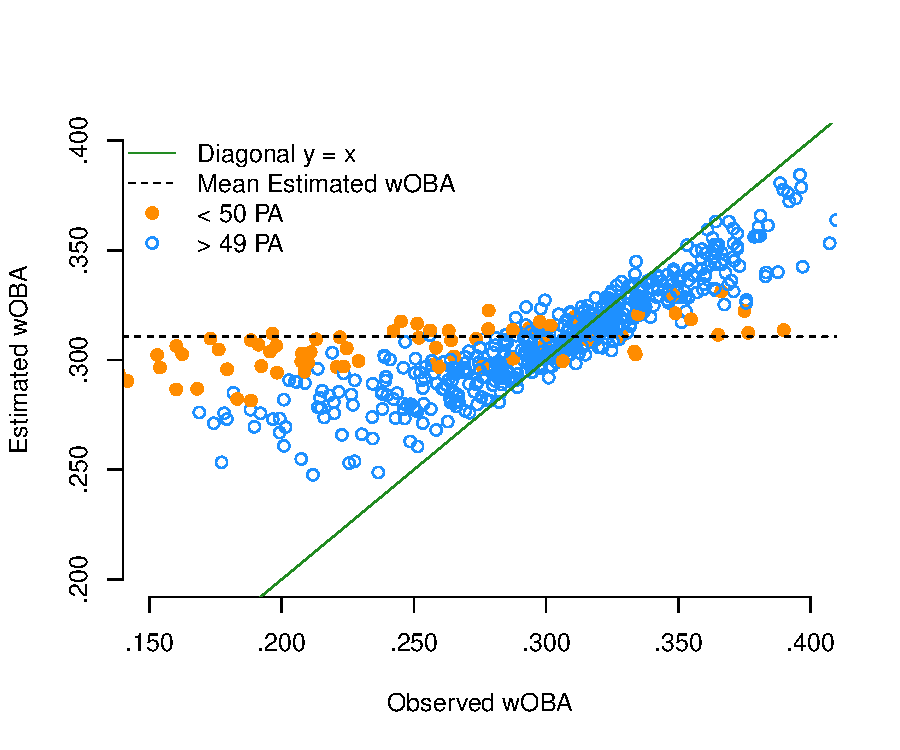
\includegraphics[width = 0.8\textwidth]
    {../figs/woba-observed-v-estimated-slides.pdf}
\end{frame}

\begin{frame}{Projected change in wOBA vs. BABIP}
\centering
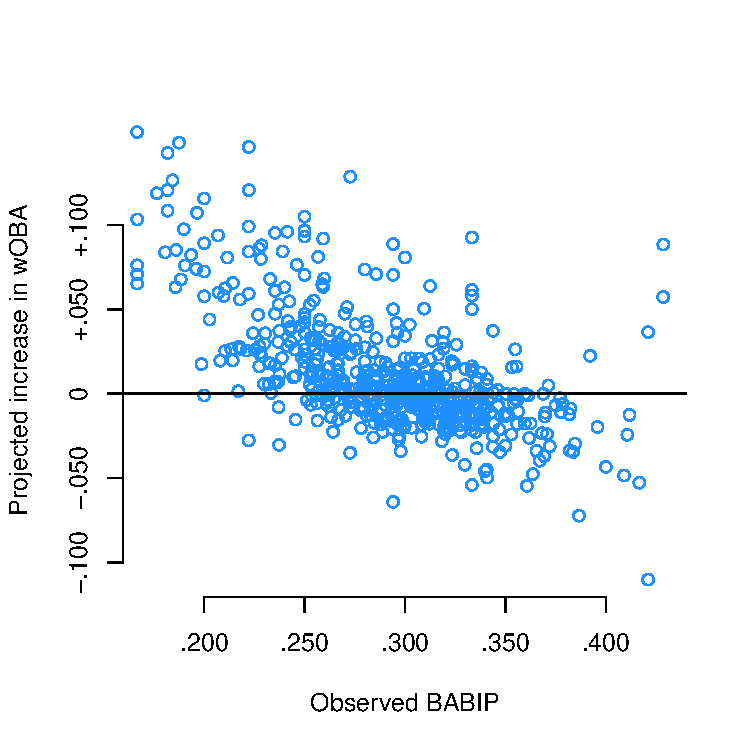
\includegraphics[width = 0.7\textwidth]{../figs/woba-v-babip-slides.pdf}
\end{frame}

\begin{frame}
\centering\Huge Methods
\end{frame}

\begin{frame}{A simple linear model}
~{\bf Data}:\\
For plate appearance $i \in \{1, ..., n\}$,\\~\\
$K_i = \l\{\begin{array}{l}1\mbox{ if $i^{th}$ PA results in strikeout}\\
    0\mbox{ otherwise}\end{array}\r.$\\~\\
$B_i =$ identity of batter in $i^{th}$ PA (e.g. Paul Goldschmidt)\\~\\
~{\bf Model}:
$$K_i = \alpha + \beta_{B_i} + \epsilon_i, \hspace{4mm}
    \mbox{where}\hspace{4mm} \epsilon_i \iid \N(0,\sigma^2)$$
~{\bf Estimator}:
$$(\hat\alpha, \hat\beta) = \arg\min\sum_{i=1}^n(K_i - \alpha - \beta_{B_i})^2
    \hspace{4mm} \Rightarrow \hspace{4mm}
    \hat\alpha + \hat\beta_{B} = \frac{\sum_{i:B_i=B}K_i}{\sum_{i:B_i=B}1}$$
\end{frame}

\begin{frame}{Ridge regression}
\vspace{-1cm}
\begin{align*}
\mbox{Instead of solving}&\\   (\hat\alpha, \hat\beta) = & \hspace{1mm}
    \arg\min\sum_{i=1}^n(K_i - \alpha - \beta_{B_i})^2,\\
\mbox{let's try solving}&\\    (\alpha^*, \beta^*) = & \hspace{1mm}
    \arg\min\sum_{i=1}^n(K_i-\alpha-\beta_{B_i})^2 + \lambda\sum_B\beta_B^2,
    \hspace{4mm}\lambda > 0.
\end{align*}
The result is
$$\beta^*_B = \frac{\lambda\cdot0 + n_B\hat\beta_B}{\lambda + n_B},\hspace{4mm}
    \mbox{where}\hspace{4mm}n_B = \sum_{i:B_i=B}1$$
For $\lambda = \sigma^2_L/\sigma^2_T$, this is regression to the mean!
\end{frame}

\begin{frame}{Logistic regression}
~{\bf A better model}:
$$\eta_i = \alpha + \beta_{B_i}, \hspace{4mm}\mbox{and}\hspace{4mm}
\mP(K_i = 1|\eta_i) = e^{\eta_i}/(1+e^{\eta_i})$$
\begin{center}
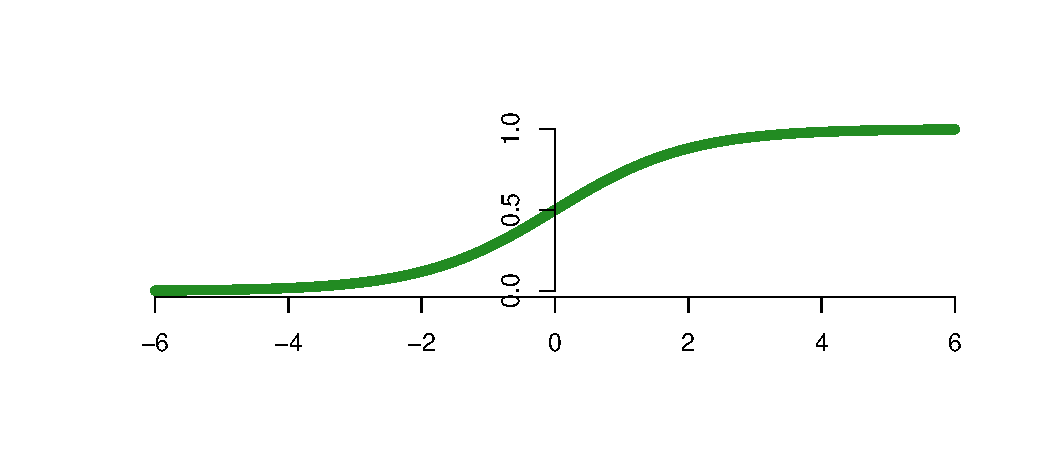
\includegraphics[width = 0.6\textwidth]{../figs/logistic.pdf}
\end{center}
~{\bf Estimator (Ridge)}:
$$(\alpha^*, \beta^*) = \arg\min-\sum_{i=1}^n\log\mP(K_i|\eta_i) +
    \lambda\sum_B\beta_B^2$$
\end{frame}

\begin{frame}{Ridge estimator vs. Naive estimator for 1B rate}
\centering
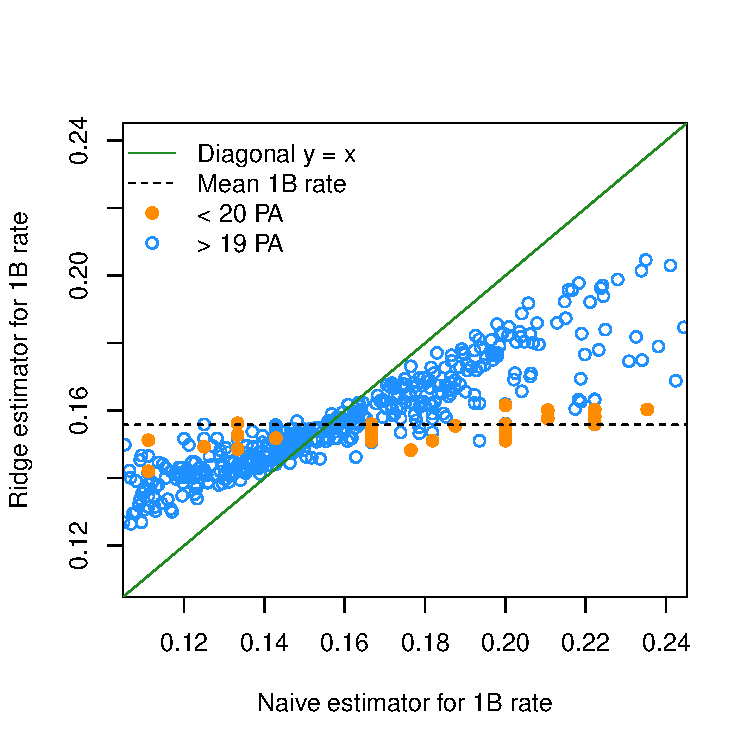
\includegraphics[width = 0.7\textwidth]{../figs/regul-as-regre-b.pdf}
\end{frame}

\begin{frame}{Ridge estimator vs. Regressed estimator for 1B rate}
\centering
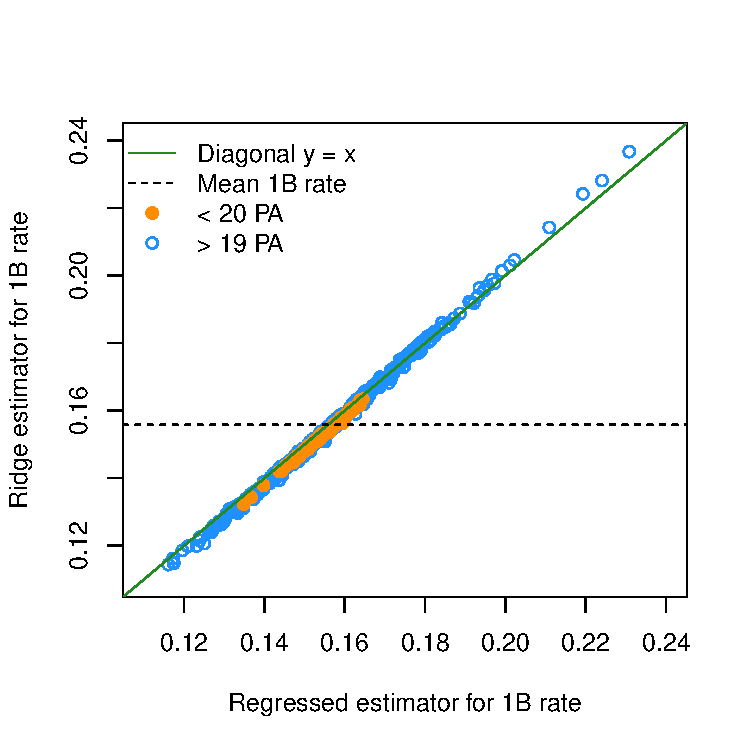
\includegraphics[width = 0.7\textwidth]{../figs/regul-as-regre-c.pdf}
\end{frame}

\begin{frame}{Test RMSE: regularization vs. regression to the mean}
\centering
\begin{tabular}{c|ccc}
    & Naive & Regressed & Ridge\\
    \hline
G   & 4.41  & 3.98      & 3.97\\
F   & 4.45  & 3.97      & 3.99\\
K   & 4.25  & 3.89      & 3.90\\
BB  & 2.60  & 2.38      & 2.39\\
HBP & 1.04  & 0.89      & 0.88\\
1B  & 3.66  & 3.09      & 3.08\\
2B  & 2.21  & 1.68      & 1.67\\
3B  & 0.82  & 0.63      & 0.64\\
HR  & 1.71  & 1.52      & 1.51
\end{tabular}\\
\vspace{1cm}
{\bf Upshot}: Ridge regression is essentially regression to the mean,\\
but it allows extensions, which we will see next!
\end{frame}

\begin{frame}{True wOBA}
~{\bf Data}:\\
$Y_i \in \Y = \{\mbox{G, F, K, BB, HBP, 1B, 2B, 3B, HR}\}$\\
$B_i =$ identity of {\bf B}atter in $i^{th}$ PA (e.g. Paul Goldschmidt)\\
$P_i =$ identity of {\bf P}itcher in $i^{th}$ PA (e.g. Zach Greinke)\\
$S_i =$ identity of {\bf S}tadium in $i^{th}$ PA (e.g. Chase Field)\\
$H_i =$ 1 if $B_i$ is on {\bf H}ome team, 0 otherwise\\
$O_i =$ 1 if $B_i$ and $P_i$ have {\bf O}pposite handedness, 0 otherwise\\~\\
~{\bf Model (multinomial logistic regression)}:
$$\eta_{ik} = \alpha_k + \beta_{B_ik} + \gamma_{P_ik} +
    \delta_{S_ik} + \zeta_kH_i + \theta_kO_i$$
$$\mP(Y_i=k|\eta_i) = \frac{e^{\eta_{ik}}}{\sum_{\ell\in\Y}e^{\eta_{i\ell}}}$$
\end{frame}

\begin{frame}{True wOBA}
~{\bf Estimation}:
\begin{align*}
\min&\l\{-\sum_{i=1}^n\mP(Y_i|\eta_i)\r.\\
    &\hspace{4mm} + \l.\sum_{k\in\Y}\lambda_k\l(\sum_B\beta_{Bk}^2
    + \sum_P\gamma_{Pk}^2 + \sum_S\delta_{Sk}^2 + \zeta_k^2 + \theta_k^2\r)\r\}
\end{align*}
\begin{itemize}
    \item Choose $\lambda_k$ via cross validation
    \item For batter $B$, estimated K rate in average situation is
    $$\mP_B(K) = \frac{e^{\alpha^*_K + \beta^*_{BK} + \frac12\zeta^*_K +
    \frac12\theta^*_K}}{\sum_{\ell\in\Y}e^{\alpha^*_\ell + \beta^*_{B\ell} +
    \frac12\zeta^*_\ell + \frac12\theta^*_\ell}}$$
    \item Combine rates of outcomes into True wOBA estimate
\end{itemize}
\end{frame}

\begin{frame}{Random effect model}
~{\bf Model}:
$$\eta_i = \alpha + \beta_{B_i}, \hspace{4mm}\mbox{where}\hspace{4mm}
\beta_B \iid \N(0, \sigma^2_\beta)$$
$$\mP(K_i = 1|\eta_i) = \Phi(\eta_i) \leftarrow \mbox{Normal CDF}$$
\begin{center}
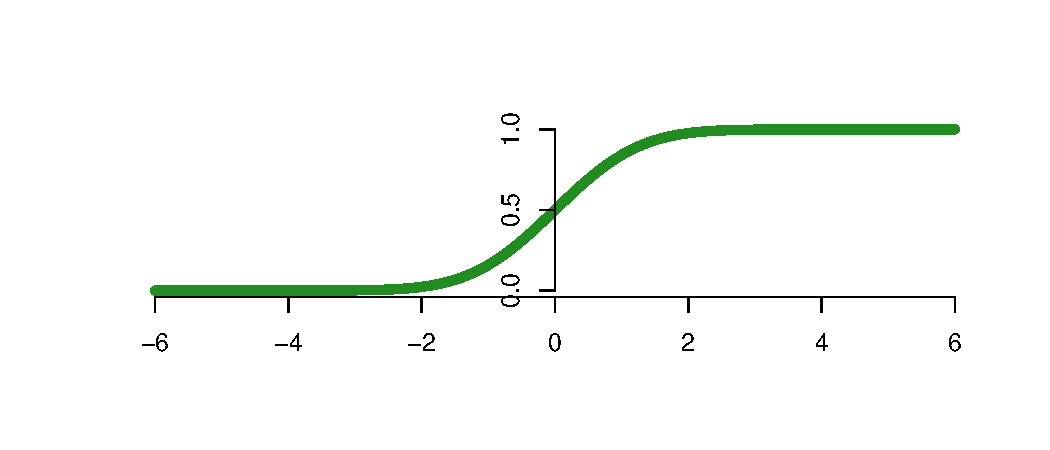
\includegraphics[width = 0.6\textwidth]{../figs/normalcdf.pdf}
\end{center}
~{\bf Estimator (Random)}:
$$(\alpha^*, \beta^*, \sigma^{2*}_\beta) =
    \arg\max L(\alpha, \beta, \sigma^2_\beta|B_i, K_i)$$
\end{frame}

\begin{frame}{Test RMSE: regularization vs. random effect model}
\begin{center}
\begin{tabular}{c|cc}
    & Regressed & Random\\
    \hline
G   & 3.38      & 3.38\\
F   & 3.48      & 3.49\\
K   & 3.30      & 3.35\\
BB  & 2.06      & 2.06\\
HBP & 0.78      & 0.77\\
1B  & 2.63      & 2.64\\
2B  & 1.45      & 1.44\\
3B  & 0.55      & 0.56\\
HR  & 1.36      & 1.35
\end{tabular}
\end{center}
{\bf Upshot}: Regularization is very similar to random effect modelling, with
two differences:
\begin{itemize}
    \item How population variance is estimated
    \item Regularization can be applied to multinomial regression
\end{itemize}
\end{frame}

\begin{frame}
\centering\Huge Results
\end{frame}

\begin{frame}{Validation}
\begin{itemize}
\item Evaluate results on 2015 MLB regular season PAs
\begin{itemize}
    \item Discard intentional walks, catcher interferences
    \item Discard PAs in which pitcher is batting
\end{itemize}
\item Fit each method on training set to predict wOBA in test set
\begin{itemize}
    \item $\{O_i = 0\} \Rightarrow$ training set with prob. 90\%
    \item $\{O_i = 1\} \Rightarrow$ test set with prob. 90\%
\end{itemize}
\item Training set: 93,868 PAs
\item Test set: 82,692 PAs
\end{itemize}
\begin{center}
\begin{tabular}{c|rrrr}
Estimator           &  Naive    & Regressed & True          & Mixed\\
\hline
Estimated MSE      & 0.00456   & 0.00220   & {\bf 0.00173} & 0.00180\\
Stadard error       &$\pm$0.00044&$\pm$0.00018&$\pm$0.00014 &$\pm$0.00015
\end{tabular}
\end{center}
\end{frame}

\begin{frame}{True wOBA vs. naive wOBA}
\centering
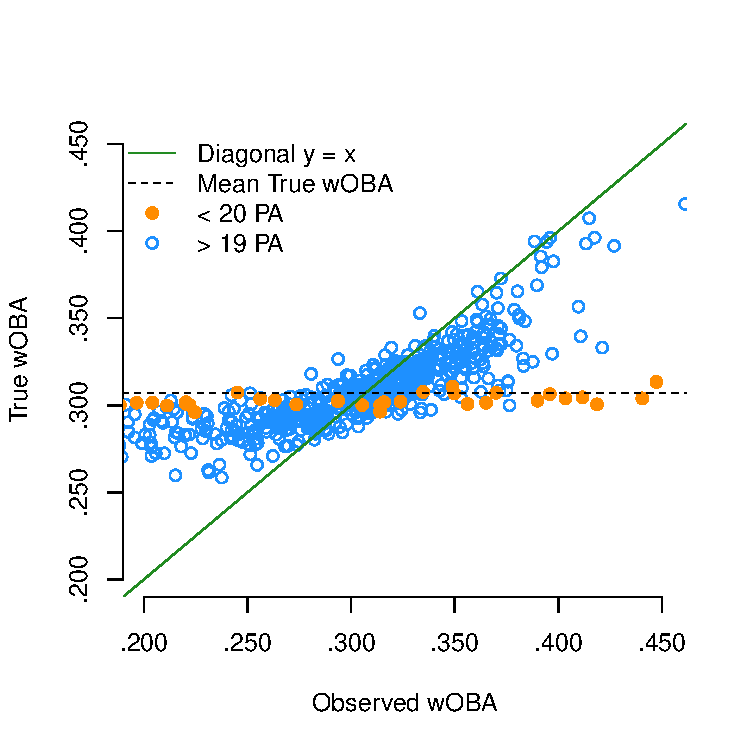
\includegraphics[width = 0.7\textwidth]{../figs/true-woba-batters.pdf}
\end{frame}

\begin{frame}{True wOBA against vs. naive wOBA against}
\centering
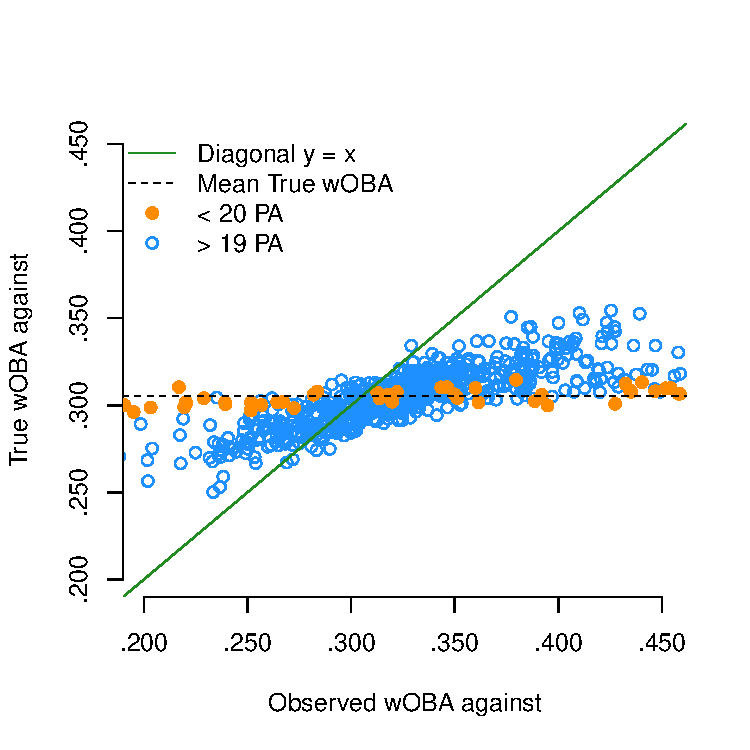
\includegraphics[width = 0.7\textwidth]{../figs/true-woba-pitchers.pdf}
\end{frame}

\begin{frame}{Top 5 and bottom 5 batters by True wOBA}
\centering
\scriptsize
\hspace*{-1cm}
\begin{tabular}{c|ccc}
      &Batter        &Team& True wOBA \\
\hline
      &Bryce Harper     &WSN & .416 \\
Top   &Mike Trout       &LAA & .407 \\
5     &Jos\'{e} Bautista&TOR & .399 \\
      &Paul Goldschmidt &ARI & .395 \\
      &Joey Votto       &CIN & .393 \\
      &...              &    &      \\*
      &Alexi Amarista   &SDP & .270 \\
Bottom&Chris Owings     &ARI & .269 \\
5     &Ren\'{e} Rivera  &TBR & .265 \\
      &Danny Santana    &MIN & .265 \\
      &Omar Infante     &KCR & .262 
\end{tabular}
\end{frame}

\begin{frame}{Top 5 and bottom 5 pitchers by True wOBA against}
\centering
\scriptsize
\hspace*{-1cm}
\begin{tabular}{c|ccc}
      & Pitcher    &Team& True wOBA against\\
\hline
      &Jake Arrieta   &CHC & .255 \\
Top   &Clayton Kershaw&LAD & .256 \\
5     &Zack Greinke   &LAD & .261 \\
      &Wade Davis     &KCR & .267 \\
      &Dallas Keuchel &HOU & .267 \\
      &...            &    &      \\
      &Jeremy Guthrie &KCR & .346 \\
Bottom&Matt Boyd      &DET & .346 \\
5     &David Holmberg &CIN & .349 \\
      &Dustin McGowan &PHI & .354 \\
      &Allen Webster  &ARI & .356
\end{tabular}
\end{frame}

\begin{frame}{Top differences between naive and True wOBA}
\centering
\scriptsize
\hspace*{-0.5cm}
\begin{tabular}{c|ccc}
      &Batter      &Team& $\Delta$wOBA\\
\hline
      &Wilson Ramos    &WSN & +.022\\
Top   &Michael Taylor  &WSN & +.021\\
5     &Albert Pujols   &LAA & +.017\\
      &Alcides Escobar &KCR & +.016\\
      &Chris Owings    &ARI & +.014\\
      & ...            &    &      \\
      &Anthony Rizzo   &CHC &--.035\\
Bottom&Nolan Arenado   &COL &--.037\\
5     &Charlie Blackmon&COL &--.039\\
      &Bryce Harper    &WSN &--.045\\
      &David Peralta   &ARI &--.046
\end{tabular}
\end{frame}

\begin{frame}{Top differences between naive and True wOBA against}
\centering
\scriptsize
\hspace*{-0.5cm}
\begin{tabular}{c|ccc}
      &Pitcher     &Team&$\Delta$wOBA against\\
\hline
      &Chris Rusin    &COL &--.068\\
Top   &Kyle Kendrick  &COL &--.062\\
5     &Jerome Williams&PHI &--.047\\
      &Matt Garza     &MIL &--.045\\
      &Kyle Lohse     &MIL &--.041\\
      &...            &    &      \\
      &Jacob deGrom   &NYM & +.016\\
Bottom&Sonny Gray     &OAK & +.016\\
5     &Clayton Kershaw&LAD & +.019\\
      &Jake Arrieta   &CHC & +.021\\
      &Zack Greinke   &LAD & +.023
\end{tabular}
\end{frame}

\begin{frame}{Discussion}
Three contributions:
\begin{itemize}
\item We advocate use of regression to the mean instead of stabilization rates
\item We explain relationship between regularized linear models and regression
    to the mean
\item We compare regularized linear models with linear mixed effects models
\end{itemize}
\end{frame}

\begin{frame}{Thank you!}
\centering
\Huge Questions?\\~\\
\normalsize
Scott Powers            \hfill  Eli Shayer\\
sspowers@stanford.edu   \hfill  eshayer@stanford.edu\\
                        \hfill  elishayer.com\\~\\
{\tt github.com/sspowers/true-woba}\\~\\
{\tt stanfordsportsanalytics.com}\\
\hfill
\includegraphics[width = 1in]{../figs/ssac.png}
\end{frame}

\end{document}
